% !TEX program = xelatex
\documentclass[aspectratio=169]{beamer}
\usepackage{amsmath}
\usepackage{amssymb}
\usepackage{graphicx}
\usepackage{tcolorbox}
\usepackage{booktabs}
\usepackage{colortbl}
\usepackage{xcolor}
\usepackage{tikz}
\usetikzlibrary{angles,quotes}
\usepackage[utf8]{inputenc}

% Custom colors
\definecolor{primary}{RGB}{41, 128, 185}
\definecolor{secondary}{RGB}{52, 152, 219}
\definecolor{accent}{RGB}{231, 76, 60}
\definecolor{lightgray}{RGB}{236, 240, 241}

% Theme customization
\usetheme{Madrid}
\usecolortheme{whale}
\setbeamercolor{structure}{fg=primary}
\setbeamercolor{background canvas}{bg=white}
\setbeamercolor{normal text}{fg=black}

% Title page info
\title{Pre-Calculus 11}
\subtitle{The Ambiguous Case of the Sine Law}
\author{Created by Yi-Chen Lin}
\date{\today}

\begin{document}

% Title Page
\begin{frame}
    \titlepage
\end{frame}

% What is the Ambiguous Case?
\begin{frame}{What is the Ambiguous Case?}
    \begin{tcolorbox}[colback=lightgray,colframe=primary,title=What is the Ambiguous Case?]
        \footnotesize
        \begin{itemize}
            \item The ambiguous case occurs when using the Sine Law to solve a triangle and two different triangles can be constructed with the given information.
            \item This happens when you are given two sides and a non-included angle (SSA case), and the side opposite the given angle is shorter than the other given side.
            \item You must consider both possible triangles.
        \end{itemize}
    \end{tcolorbox}
    
    \vspace{0.5em}
    \begin{center}
    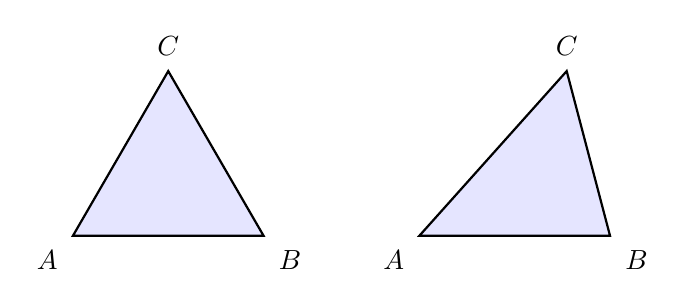
\begin{tikzpicture}[scale=1.1]
        % First triangle (left)
        \coordinate (A) at (0,0);
        \coordinate (B) at (2.2,0);
        \coordinate (C) at (1.1,1.9);
        \fill[blue!10] (A) -- (B) -- (C) -- cycle;
        \draw[thick] (A) -- (B) -- (C) -- cycle;
        % Vertices only
        \node[below left=2pt] at (A) {$A$};
        \node[below right=2pt] at (B) {$B$};
        \node[above=2pt] at (C) {$C$};
        % No side or angle labels
        % Second triangle (right)
        \begin{scope}[xshift=4cm]
            \coordinate (A2) at (0,0);
            \coordinate (B2) at (2.2,0);
            \coordinate (C2) at (1.7,1.9);
            \fill[blue!10] (A2) -- (B2) -- (C2) -- cycle;
            \draw[thick] (A2) -- (B2) -- (C2) -- cycle;
            % Vertices only
            \node[below left=2pt] at (A2) {$A$};
            \node[below right=2pt] at (B2) {$B$};
            \node[above=2pt] at (C2) {$C$};
            % No side or angle labels
        \end{scope}
    \end{tikzpicture}
    \end{center}
    \vspace{0.5em}
    \footnotesize
    A second triangle that meets these specs can be made by making an isosceles triangle inside the first one. An ambiguous case will occur when we have two different triangles that can meet the given requirements.
\end{frame}

% Example: Two Possible Triangles (side by side, matching sample)
\begin{frame}{Example: Two Possible Triangles}
    \begin{tcolorbox}[colback=lightgray,colframe=primary,title=Question]
        \footnotesize
        In $\triangle ABC$, $A = 30^\circ$, $a = 10$, $c = 16$. Find all possible values for $B$ and $b$.
    \end{tcolorbox}
    \vspace{1em}
    \begin{center}
    \begin{tikzpicture}[scale=1.1]
        % First triangle (left)
        \coordinate (A) at (0,0);
        \coordinate (B) at (2.2,0);
        \coordinate (C) at (1.1,1.9);
        \fill[blue!10] (A) -- (B) -- (C) -- cycle;
        \draw[thick] (A) -- (B) -- (C) -- cycle;
        \node[below left=2pt] at (A) {$A=30^\circ$};
        \node[below right=2pt] at (B) {$B$};
        \node[above=2pt] at (C) {$C$};
        \node[font=\small] at ($(A)!0.5!(C)$) {16};
        \node[font=\small] at ($(B)!0.5!(C)$) {10};
        % Second triangle (right)
        \begin{scope}[xshift=4cm]
            \coordinate (A2) at (0,0);
            \coordinate (B2) at (2.2,0);
            \coordinate (C2) at (1.7,1.9);
            \fill[blue!10] (A2) -- (B2) -- (C2) -- cycle;
            \draw[thick] (A2) -- (B2) -- (C2) -- cycle;
            \node[below left=2pt] at (A2) {$A=30^\circ$};
            \node[below right=2pt] at (B2) {$B$};
            \node[above=2pt] at (C2) {$C$};
            \node[font=\small] at ($(A2)!0.5!(C2)$) {16};
            \node[font=\small] at ($(B2)!0.5!(C2)$) {10};
        \end{scope}
    \end{tikzpicture}
    \end{center}
\end{frame}

\begin{frame}{Example: Two Possible Triangles}
    \begin{tcolorbox}[colback=lightgray,colframe=primary,title=Solution (Triangle 1)]
        \footnotesize
        \begin{columns}
            \column{0.55\textwidth}
            \begin{align*}
                \frac{a}{\sin A} &= \frac{c}{\sin C} \\
                \frac{10}{\sin 30^\circ} &= \frac{16}{\sin C} \\
                \sin C &= \frac{16 \cdot \sin 30^\circ}{10} = 0.8 \\
                C_1 &= \sin^{-1}(0.8) \approx 53.13^\circ \\
                B_1 &= 180^\circ - 30^\circ - 53.13^\circ = 96.87^\circ \\
                \frac{a}{\sin A} &= \frac{b_1}{\sin B_1} \\
                b_1 &= \frac{10 \cdot \sin 96.87^\circ}{\sin 30^\circ} \approx 19.93
            \end{align*}
            \column{0.45\textwidth}
            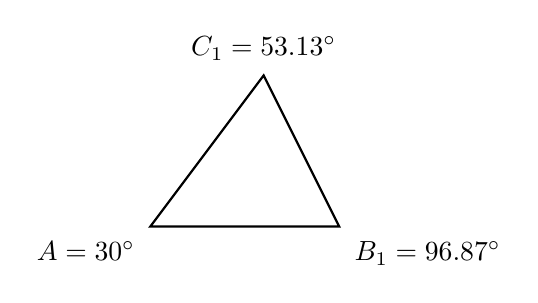
\begin{tikzpicture}[scale=0.6]
                \coordinate (A) at (0,0);
                \coordinate (B) at (4,0);
                \coordinate (C) at ({4*cos(53.13)},{4*sin(53.13)});
                \draw[thick] (A) -- (B) -- (C) -- cycle;
                \node[below left=2pt] at (A) {$A=30^\circ$};
                \node[below right=2pt] at (B) {$B_1=96.87^\circ$};
                \node[above=2pt] at (C) {$C_1=53.13^\circ$};
            \end{tikzpicture}
        \end{columns}
    \end{tcolorbox}
\end{frame}

\begin{frame}{Example: Two Possible Triangles}
    \begin{tcolorbox}[colback=lightgray,colframe=primary,title=Solution (Triangle 2)]
        \footnotesize
        \begin{columns}
            \column{0.55\textwidth}
            \begin{align*}
                C_2 &= 180^\circ - 53.13^\circ = 126.87^\circ \\
                B_2 &= 180^\circ - 30^\circ - 126.87^\circ = 23.13^\circ \\
                b_2 &= \frac{10 \cdot \sin 23.13^\circ}{\sin 30^\circ} \approx 7.86
            \end{align*}
            \column{0.45\textwidth}
            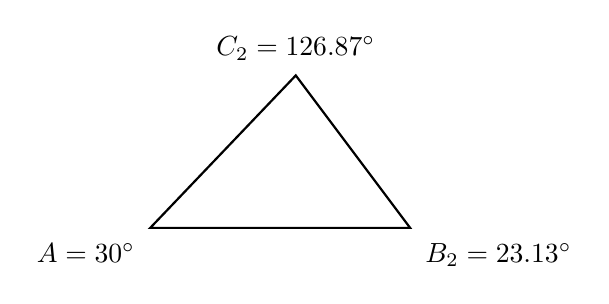
\begin{tikzpicture}[scale=1.1]
                % Vertices
                \coordinate (A) at (0,0);
                \coordinate (B) at (3,0);
                \coordinate (C) at ({3+2.2*cos(126.87)},{2.2*sin(126.87)});
                \draw[thick] (A) -- (B) -- (C) -- cycle;
                % Angle labels
                \node[below left=2pt] at (A) {$A=30^\circ$};
                \node[below right=2pt] at (B) {$B_2=23.13^\circ$};
                \node[above=2pt] at (C) {$C_2=126.87^\circ$};
            \end{tikzpicture}
        \end{columns}
    \end{tcolorbox}
\end{frame}

% Practice: Ambiguous Case
\begin{frame}{Practice: Ambiguous Case}
    \begin{tcolorbox}[colback=lightgray,colframe=accent,title=Practice]
        \footnotesize
        In $\triangle ABC$, $A = 48^\circ$, $a = 9$, $c = 11$. Find all possible values for $B$ and $C$.
    \end{tcolorbox}
\end{frame}

\begin{frame}{Practice: Ambiguous Case}
    \begin{tcolorbox}[colback=lightgray,colframe=accent,title=Solution (Triangle 1)]
        \footnotesize
        \begin{columns}
            \column{0.55\textwidth}
            \begin{align*}
                \frac{a}{\sin A} &= \frac{c}{\sin C} \\
                \frac{9}{\sin 48^\circ} &= \frac{11}{\sin C} \\
                \sin C &= \frac{11 \cdot \sin 48^\circ}{9} \approx 0.914 \\
                C_1 &= \sin^{-1}(0.914) \approx 66.73^\circ \\
                B_1 &= 180^\circ - 48^\circ - 66.73^\circ = 65.27^\circ
            \end{align*}
            \column{0.45\textwidth}
            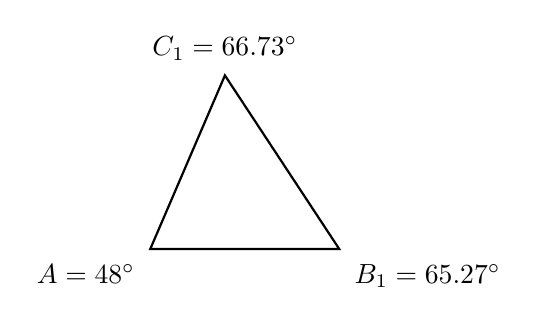
\begin{tikzpicture}[scale=0.6]
                \coordinate (A) at (0,0);
                \coordinate (B) at (4,0);
                \coordinate (C) at ({4*cos(66.73)},{4*sin(66.73)});
                \draw[thick] (A) -- (B) -- (C) -- cycle;
                \node[below left=2pt] at (A) {$A=48^\circ$};
                \node[below right=2pt] at (B) {$B_1=65.27^\circ$};
                \node[above=2pt] at (C) {$C_1=66.73^\circ$};
            \end{tikzpicture}
        \end{columns}
    \end{tcolorbox}
\end{frame}

\begin{frame}{Practice: Ambiguous Case}
    \begin{tcolorbox}[colback=lightgray,colframe=accent,title=Solution (Triangle 2)]
        \footnotesize
        \begin{columns}
            \column{0.55\textwidth}
            \begin{align*}
                C_2 &= 180^\circ - 66.73^\circ = 113.27^\circ \\
                B_2 &= 180^\circ - 48^\circ - 113.27^\circ = 18.73^\circ
            \end{align*}
            \column{0.45\textwidth}
            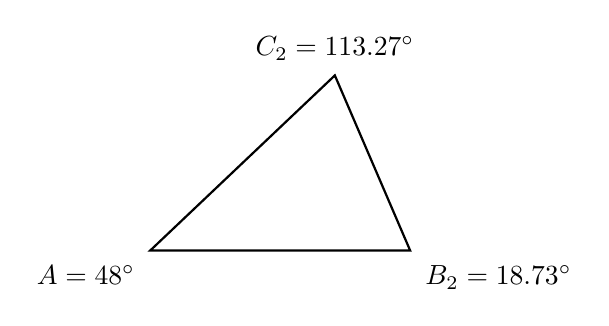
\begin{tikzpicture}[scale=1.1]
                % Vertices
                \coordinate (A) at (0,0);
                \coordinate (B) at (3,0);
                \coordinate (C) at ({3+2.2*cos(113.27)},{2.2*sin(113.27)});
                \draw[thick] (A) -- (B) -- (C) -- cycle;
                % Angle labels
                \node[below left=2pt] at (A) {$A=48^\circ$};
                \node[below right=2pt] at (B) {$B_2=18.73^\circ$};
                \node[above=2pt] at (C) {$C_2=113.27^\circ$};
            \end{tikzpicture}
        \end{columns}
    \end{tcolorbox}
\end{frame}

% When is the Ambiguous Case Possible?
\begin{frame}{When is the Ambiguous Case Possible?}
    \begin{tcolorbox}[colback=lightgray,colframe=primary,title=Summary]
        \footnotesize
        \begin{itemize}
            \item The ambiguous case (SSA) is possible when:
            \begin{itemize}
                \item The side opposite the given angle is shorter than the other given side, but longer than the height from the given angle.
                \item $a < c$ and $a > c \sin A$
            \end{itemize}
            \item If the side opposite the angle is longer than the other given side, only one triangle is possible.
            \item If the side opposite the angle is shorter than the height, no triangle is possible.
        \end{itemize}
    \end{tcolorbox}
\end{frame}

\end{document} 